\documentclass[11pt]{article}
\usepackage[utf8]{inputenc}
\usepackage{amsmath,amssymb}
\usepackage{graphicx}
\usepackage{booktabs}
\usepackage{authblk}
\usepackage[margin=1in]{geometry}
\usepackage[hidelinks]{hyperref}
\usepackage{xurl}
\usepackage{setspace}
\usepackage{tikz}
\usetikzlibrary{arrows.meta,positioning}

\title{Solar Fusion by Coulomb Alone}
\author[1]{Claes Johnson}
\affil[1]{KTH Royal Institute of Technology, SE-100 44 Stockholm, Sweden \\
\texttt{claesjohnson@gmail.com}}
\date{\today \\[0.4em]
\small\textit{Physical argument by the author; numerical implementation with AI assistance (Claude, Anthropic).}}

\begin{document}
\maketitle

\begin{abstract}
We argue that the Sun shines by \emph{Coulomb forces alone}: solar hydrogen burning can be carried
through entirely by the electrostatic attraction between protons and electrons, with no strong and no
weak force, and --- in the relativity-free formulation adopted here --- no appeal even to $E=mc^2$. In
the standard proton--proton chain, by contrast, the burning begins with $p+p\to d+e^{+}+\nu_e$, a
\emph{weak}-force reaction that converts a proton into a neutron with emission of a positron and a
neutrino, and is the slow, rate-limiting step of the whole chain. In the RealNucleus picture --- in
which the neutron is a bound proton--electron pair and the deuteron is $2p+1e$ --- the same first step
is purely \emph{electromagnetic}: $p+e+p\to d$, an electron from the plasma captured as the deuteron's
glue, with no flavour change, no positron, and no neutrino. Two deuterons then fuse to the alpha,
$d+d\to{}^4$He, a reaction computed directly in RealQM. The net process $4p+2e\to{}^4\mathrm{He}$
releases the same ${\sim}26.7$~MeV as the standard chain but retains the ${\sim}0.5$~MeV per alpha
(${\sim}2\%$) that the standard chain loses to neutrinos. The difference is a lepton one: in RealNucleus
no lepton is created or destroyed --- the electron persists as the deuteron's constituent --- so the
electromagnetic route \emph{requires} no neutrino, whereas the standard neutrino is the signature of the
flavour-changing weak vertex $p\to n$. We stress the scope explicitly: this is a statement about the
\emph{mechanism} only. RealNucleus says nothing about neutrinos as such --- in particular it does
\emph{not} claim that neutrinos do not exist, and it makes \emph{no} prediction for the solar neutrino
flux. It exhibits a Coulomb route to fusion that needs no neutrino; where the neutrinos observed from
the Sun originate is a question outside the model's scope, on which it is silent. This second version is formulated \emph{without relativity}: all energies are taken as
directly measured --- photon energies, reaction $Q$-values, photodisintegration thresholds --- rather
than inferred from mass deficits, so the energetics owe nothing even to $E=mc^2$, and a directly-measured
energy release stands as the more model-free benchmark.

\medskip
\noindent\textbf{Keywords:} solar fusion; proton--proton chain; deuteron formation; electron capture;
RealNucleus; weak force; solar neutrinos; hydrogen burning.
\end{abstract}

\doublespacing

\section{Introduction}

The Sun shines by fusing \emph{hydrogen} into helium, releasing $26.73$~MeV per helium nucleus. Its
burning admits two accounts. The \emph{standard} account~\cite{Bethe,Adelberger} runs through the
proton--proton chain, whose first and rate-limiting step is a \emph{weak}-interaction conversion of a
proton into a neutron; the \emph{RealNucleus} account developed here~\cite{Johnson-RealNucleus,%
Johnson-RealQM}, in which the electron is an active constituent of every nucleus, replaces that step by
a purely \emph{electromagnetic} capture. Having named them, we may compare them; and the two differ
already in how they write the ingredients. What is consumed are hydrogen atoms --- protons \emph{and}
electrons. The standard account keeps only the protons, treating
the electrons as a passive plasma background, and writes the net as $4p\to{}^4\mathrm{He}$ (with the
plasma electrons entering later, through positron annihilation). RealNucleus, in which the electron is
an active constituent of every nucleus, keeps them explicit throughout: four hydrogen atoms,
$4\mathrm{H}=4p+4e$, become one helium atom, $(2e+4p)+2e$, i.e. the alpha $(2e+4p)$ dressed by two outer
electrons. Both net to the same $26.73$~MeV; they differ in the mechanism and in whether electrons are
bookkeeping or physics. In the standard account~\cite{Bethe,Adelberger} the burning proceeds through the
proton--proton (pp) chain, whose first and rate-limiting step,
\begin{equation}
p + p \;\longrightarrow\; d + e^{+} + \nu_e ,
\label{eq:pp}
\end{equation}
is a \emph{weak}-interaction process: two protons collide, one is converted to a neutron
($p\to n + e^{+} + \nu_e$), and the resulting proton and neutron bind as a deuteron. Because it
requires the weak force acting during the brief instant two protons are within nuclear range, this
step is extraordinarily slow --- it is what makes the Sun's hydrogen last billions of years --- and it
emits a neutrino that escapes the Sun directly.

RealNucleus~\cite{Johnson-RealNucleus,Johnson-RealQM} offers a different account of the same burning.
There the neutron is not elementary but a bound proton--electron pair, $n=(p\,e^-)$, and the deuteron
is accordingly $2p+1e$: two protons glued by a single shared electron, the charge-conjugate of the
one-electron molecular ion $\mathrm{H}_2^{+}$. In this picture the first step of hydrogen burning is
not weak but electromagnetic,
\begin{equation}
p + e + p \;\longrightarrow\; d ,
\label{eq:pep}
\end{equation}
an electron drawn from the surrounding plasma and captured as the deuteron's glue --- no proton is
converted, no positron is created, and no neutrino is required. The chain then closes with the direct
fusion of two deuterons,
\begin{equation}
d + d \;\longrightarrow\; {}^4\mathrm{He} ,
\label{eq:dd}
\end{equation}
a reaction we have computed directly in RealQM~\cite{Johnson-RealNucleus}. This paper places the two
accounts side by side and compares their energetics and their lepton content. We are careful about
scope: RealNucleus offers a Coulomb \emph{mechanism} for the burning; it makes no prediction for, and
no claim about, the solar neutrino flux, and does not assert that neutrinos do not exist
(\S\ref{sec:test}).

\section{The standard proton--proton chain}

The dominant (ppI) branch of the standard chain is
\begin{align}
p + p &\to d + e^{+} + \nu_e && (Q = 0.42~\text{MeV};\ \text{weak, rate-limiting}),\\
d + p &\to {}^3\mathrm{He} + \gamma && (Q = 5.49~\text{MeV}),\\
{}^3\mathrm{He} + {}^3\mathrm{He} &\to {}^4\mathrm{He} + 2p && (Q = 12.86~\text{MeV}),
\end{align}
with the two positrons annihilating on plasma electrons. Summing the branch and the annihilations, the
net is
\begin{equation}
4p + 2e^- \;\longrightarrow\; {}^4\mathrm{He} + 2\nu_e + 26.73~\text{MeV},
\label{eq:standard-net}
\end{equation}
of which the two neutrinos carry away, on average, ${\sim}0.5$~MeV, so that ${\sim}26.2$~MeV is
deposited as heat. The rate is set by two factors in series: the Coulomb barrier the two protons must
tunnel (the Gamow factor, steeply temperature-dependent), \emph{and} the weak matrix element for
$p\to n$ conversion during the collision. The second factor is tiny, and it is the weak bottleneck ---
not the Coulomb barrier alone --- that fixes the Sun's luminosity and lifetime. A minor variant, the
\emph{pep} reaction $p+e^-+p\to d+\nu_e$ (about $0.4\%$ of pp), captures a plasma electron instead of
emitting a positron, but is still weak and still emits a neutrino.

\begin{figure}[t]
\centering
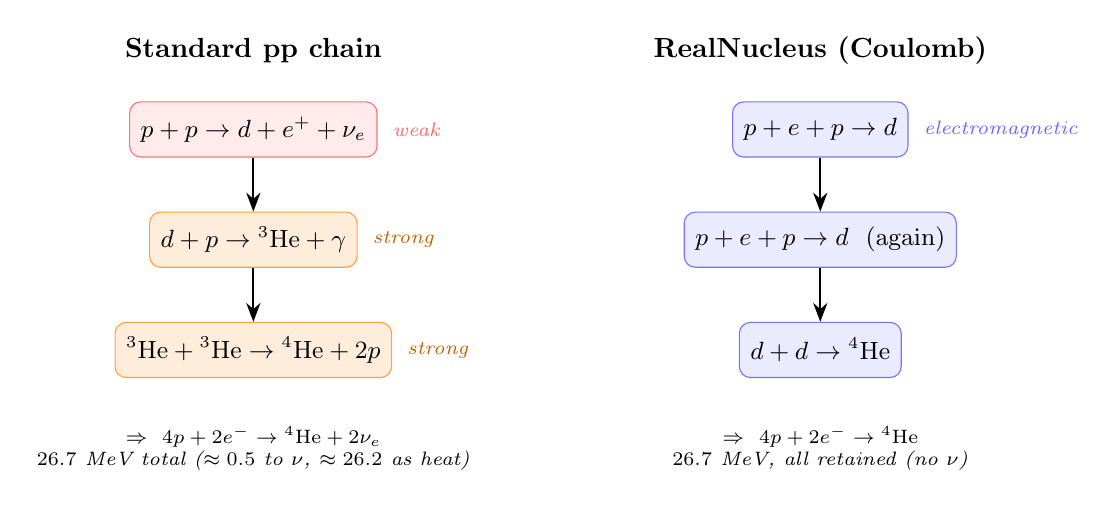
\begin{tikzpicture}[
  font=\small,
  box/.style={draw,rounded corners,inner sep=4pt,minimum height=7mm,align=center},
  wk/.style={box,fill=red!8,draw=red!55},
  st/.style={box,fill=orange!14,draw=orange!75},
  em/.style={box,fill=blue!8,draw=blue!55},
  ar/.style={-{Stealth[length=2.4mm]},thick},
  lab/.style={font=\scriptsize\itshape}]

 % ---- standard column ----
 \node[align=center,font=\bfseries] at (0,1.0) {Standard pp chain};
 \node[wk] (s1) at (0,0) {$p+p\to d+e^{+}+\nu_e$};
 \node[lab,red!60,right=2pt of s1] {weak};
 \node[st] (s2) at (0,-1.4) {$d+p\to{}^3\mathrm{He}+\gamma$};
 \node[lab,orange!75!black,right=2pt of s2] {strong};
 \node[st] (s3) at (0,-2.8) {${}^3\mathrm{He}+{}^3\mathrm{He}\to{}^4\mathrm{He}+2p$};
 \node[lab,orange!75!black,right=2pt of s3] {strong};
 \draw[ar] (s1) -- (s2);
 \draw[ar] (s2) -- (s3);
 \node[align=center,font=\scriptsize\itshape] at (0,-4.05)
   {$\Rightarrow\ 4p+2e^-\to{}^4\mathrm{He}+2\nu_e$\\ $26.7$~MeV total ($\approx0.5$ to $\nu$, $\approx26.2$ as heat)};

 % ---- RealNucleus column ----
 \node[align=center,font=\bfseries] at (7.2,1.0) {RealNucleus (Coulomb)};
 \node[em] (r1) at (7.2,0) {$p+e+p\to d$};
 \node[lab,blue!60,right=2pt of r1] {electromagnetic};
 \node[em] (r2) at (7.2,-1.4) {$p+e+p\to d$\ \ (again)};
 \node[em] (r3) at (7.2,-2.8) {$d+d\to{}^4\mathrm{He}$};
 \draw[ar] (r1) -- (r2);
 \draw[ar] (r2) -- (r3);
 \node[align=center,font=\scriptsize\itshape] at (7.2,-4.05)
   {$\Rightarrow\ 4p+2e^-\to{}^4\mathrm{He}$\\ $26.7$~MeV, all retained (no $\nu$)};
\end{tikzpicture}
\caption{The two accounts of solar hydrogen burning, colored by the force each picture assigns to each
step: \textcolor{red!70}{\textbf{red = weak}}, \textcolor{orange!80!black}{\textbf{orange = strong}},
\textcolor{blue!70}{\textbf{blue = electromagnetic}}. \emph{Left:} the standard chain opens with the
\emph{weak} reaction $p+p\to d+e^{+}+\nu_e$ (a $p\to n$ conversion emitting a neutrino), and closes with
two \emph{strong}-interaction steps, $d+p\to{}^3$He and ${}^3$He$+{}^3$He (electromagnetism enters these
only as the Coulomb barrier and the photon). \emph{Right:} the RealNucleus chain is \emph{entirely
electromagnetic} --- the capture $p+e+p\to d$ (the electron becoming the deuteron's glue), twice, then
the directly-computed $d+d\to{}^4$He; the very same reactions that are strong in the standard reading are
Coulombic here. Both routes net to the same measured $4p+2e^-\to{}^4$He release of $26.7$~MeV (a state
function, independent of path); they differ in that the standard chain loses ${\sim}0.5$~MeV to its two
neutrinos while the Coulomb route retains all of it.}
\label{fig:chains}
\end{figure}

\section{The Coulomb route}

In RealNucleus the ground state of a nucleus is a set of proton and electron charge clouds on
non-overlapping domains with free boundaries, minimising the Coulomb (electrostatic) energy alone,
\begin{equation}
E \;=\; \sum_i \tfrac{1}{2}\!\int|\nabla\psi_i|^2
\;+\; \tfrac12\!\iint\frac{\rho(x)\rho(y)}{|x-y|}\,dx\,dy, \qquad \rho=\sum_i q_i\psi_i^2 ,
\label{eq:energy}
\end{equation}
with $q_i=\pm1$~\cite{Johnson-RealQM,Johnson-RealNucleus}. A free proton and a free electron form the
model neutron $1p+1e$, which does \emph{not} bind on its own (matching the instability of the free
neutron); but a \emph{second} proton produces the deuteron $2p+1e$, which does. The single electron
cannot glue one proton into a bound unit yet glues two --- the charge-conjugate $\mathrm{H}^-$/
$\mathrm{H}_2^{+}$ configuration, the two protons splitting into halfspaces around the central electron
core. This is the reaction~\eqref{eq:pep}: it needs only an electron, always abundant in the solar
plasma, and the Coulomb attraction that binds it; no proton is transmuted.

The electron glue carries no relativity and no mass. Under the homogeneous-Neumann free-boundary
condition of RealQM the deuteron's configuration is fixed by \emph{charge continuity} --- the boundary
sits where the electron and proton densities match --- and a flat (uniform) electron core satisfies that
condition trivially, with zero gradient and hence zero kinetic energy. Its mass therefore drops out
altogether: a rigid uniform electron caged by two protons is charge-continuous with them at a definite
radius \emph{independent of the electron mass}, as verified directly~\cite{Johnson-RealNucleus}. The
femtometre scale of the deuteron is set by the heavy proton, not the light electron, which merely fills
the cage. Consistently with the relativity-free formulation of this paper, the entry step $p+e+p\to d$
thus invokes neither a mass parameter nor $E=mc^2$.

The second step~\eqref{eq:dd}, $d+d\to{}^4\mathrm{He}$, is the fusion of two such units into the alpha
$4p+2e$ --- the closed, dual-confined structure in which a $-2$ electron core is caged by four
protons. In RealQM this reaction is computed directly: two deuterons, each a central electron core
with its two protons split into halfspaces, are brought together and relaxed, and the energy falls
monotonically onto the deeply bound alpha as the separation decreases~\cite{Johnson-RealNucleus}. The
overall balance is
\begin{equation}
4p + 2e^- \;\longrightarrow\; {}^4\mathrm{He} + 26.73~\text{MeV},
\label{eq:coulomb-net}
\end{equation}
identical in energy to the standard net~\eqref{eq:standard-net} except that no energy is carried off by
neutrinos.

\paragraph{Which second step?} A caveat on abundances is in order. In the solar core protons outnumber
deuterons enormously: a deuteron, once formed, is consumed almost at once, so its equilibrium
abundance is only $[d]/[p]\sim10^{-18}$. In the standard chain this is precisely why deuterium burns by
$d+p\to{}^3\mathrm{He}$ and not by $d+d$, which is utterly negligible. The same abundance argument
applies to the Coulomb route: the dominant second step in a proton-rich plasma is likewise
$d+p\to{}^3\mathrm{He}$ --- in RealNucleus simply $3p+1e$, again electromagnetic --- followed by
${}^3\mathrm{He}+{}^3\mathrm{He}\to{}^4\mathrm{He}+2p$, exactly the ppI topology but with every step
Coulombic and neutrino-free. We write the chain as $d+d\to{}^4\mathrm{He}$ in~\eqref{eq:dd} because that
reaction is the one computed directly in RealQM~\cite{Johnson-RealNucleus} and the cleanest picture of
two dual-confined units merging into the closed alpha; the abundance-weighted path through
${}^3\mathrm{He}$ tells the same electromagnetic story, $4p+2e^-\to{}^4\mathrm{He}$, and is equally free
of the weak vertex. The essential contrast with the standard chain therefore lies entirely in the
\emph{first} step, the formation of the deuteron: whether it is the weak $p+p\to d+e^{+}+\nu_e$ or the
electromagnetic $p+e+p\to d$. Every step thereafter is Coulombic in both accounts; only the entry point
carries --- or does not carry --- the neutrino.

\section{Comparison}

Table~\ref{tab:compare} sets the two accounts against each other. They agree on the overall
transmutation and on its energy release; they differ on the \emph{mechanism} of the first step, and
hence on the leptons and the neutrinos.

\begin{table}[h]
\centering
\renewcommand{\arraystretch}{1.25}
\begin{tabular}{lll}
\toprule
 & \textbf{Standard pp chain} & \textbf{RealNucleus (Coulomb)}\\
\midrule
first step        & $p+p\to d+e^{+}+\nu_e$      & $p+e+p\to d$\\
force             & weak (flavour-changing $p\to n$) & electromagnetic (Coulomb)\\
what the deuteron is & $p+n$, $n$ elementary     & $2p+1e$, $n=(p\,e^-)$ bound\\
second step       & $d+p\to{}^3$He, then ${}^3$He$+{}^3$He & $d+d\to{}^4$He (computed)\\
leptons           & $e^{+}$ and $\nu_e$ created   & electron retained; none created\\
neutrinos         & yes ($2\,\nu_e$ per $^4$He)  & none\\
net               & $4p+2e^-\to{}^4$He$+2\nu_e$   & $4p+2e^-\to{}^4$He\\
energy            & $26.73$~MeV ($\sim0.5$ to $\nu$) & $26.73$~MeV (all retained)\\
rate limiter      & weak vertex $\times$ Coulomb barrier & Coulomb barrier (three-body $p e p$)\\
\bottomrule
\end{tabular}
\caption{The standard proton--proton chain and the RealNucleus Coulomb route to solar hydrogen
burning, step by step.}
\label{tab:compare}
\end{table}

\paragraph{The lepton argument.} The cleanest distinction is one of lepton bookkeeping. In the standard
first step a proton is turned into a neutron, a flavour-changing weak transition that must create a
positron and a neutrino to conserve charge and lepton number: the neutrino is the \emph{signature of
the weak vertex}. In the Coulomb route no proton is transmuted and no lepton is created or destroyed
--- the plasma electron simply becomes the deuteron's glue and remains as the constituent electron of
the $n=(p\,e^-)$ pair. Lepton number is then conserved trivially, with no neutrino. The presence or
absence of the solar neutrino is thus a direct readout of which mechanism operates.

\section{Energetics and the neutrino budget}

Both routes effect the same net transmutation $4p+2e^-\to{}^4\mathrm{He}$ and release the same
$26.73$~MeV. Throughout this paper we take such energies as \emph{directly measured} --- calorimetrically,
as the heat and radiation the reactions give up, and as the reaction energies read from emitted gamma
rays, particle kinetic energies, and photodisintegration thresholds --- and we do not invoke any
mass--energy relation or any relativity. Binding energies here are not mass deficits: the deuteron
binding, for instance, is the $2.22$~MeV \emph{capture gamma} of $n+p\to d+\gamma$, read straight off a
spectrometer, and the neutron's $0.78$~MeV excess over $p+e$ is its beta-decay endpoint. A
directly-measured energy release is, if anything, the more model-free benchmark, owing nothing even to
$E=mc^2$.

It is worth seeing where this energy is actually generated, because in the Coulomb route the two steps
are very unequal. Forming the two deuterons releases little: each deuteron sits only $1.44$~MeV below
$2p+e$ (the $2.22$~MeV capture gamma against $p+n$, less the neutron's $0.78$~MeV beta endpoint, leaves
$1.44$~MeV against protons and electrons), so the two formations contribute $2\times1.44\approx2.9$~MeV,
about $11\%$ of the total. The overwhelming balance comes from the fusion of the two deuterons into the
alpha,
\begin{equation}
d + d \to {}^4\mathrm{He}: \qquad \approx 23.8~\text{MeV} \;\; (\approx 89\%),
\end{equation}
this being the alpha's binding relative to two deuterons, again a directly-measured reaction energy,
where the two loosely-bound $2p+1e$ units merge into the deeply-bound $2e+4p$ alpha --- the two electron
cores settling into a single $-2$ glue now caged by \emph{four} protons instead of two. The Sun's
luminosity is therefore, to $\sim\!89\%$, the \emph{alpha-binding energy}: deuteron formation is only
the small doorway, and $d+d\to{}^4\mathrm{He}$ is the powerhouse. This dominant term is not only
directly measured but directly \emph{computed}: in RealNucleus the alpha binds at $29.1$~MeV against the
experimental $28.3$ ($103\%$), from the single deuteron-calibrated scale and with nothing else
fitted~\cite{Johnson-RealNucleus}, so the ${\sim}89\%$ of the solar output that is the alpha binding is
reproduced by the Coulomb model itself, not merely taken from experiment. (In the Sun the abundance-weighted
path reaches the alpha through $d+p\to{}^3\mathrm{He}$ and ${}^3\mathrm{He}+{}^3\mathrm{He}$ rather than
$d+d$, since deuterium is consumed by protons far faster; the total is the same state-function
$26.73$~MeV, only distributed differently.)

The standard chain gives up about $0.5$~MeV of this to its two neutrinos (mean pp-neutrino energy
$\approx 0.27$~MeV each), so $\approx 26.2$~MeV becomes solar heat and light; the Coulomb route retains
the full $26.73$~MeV. Equivalently, the standard model predicts a solar \emph{neutrino luminosity} of
about $2\%$ of the total, while the Coulomb route predicts essentially none. This few-percent split is
small in the energy budget but it is the whole of the observable neutrino signal.

\section{On solar neutrinos: the scope of the claim}
\label{sec:test}

It is essential to state precisely what is, and is not, claimed. Solar neutrinos are \emph{observed} ---
the chlorine and gallium radiochemical experiments, Super-Kamiokande and SNO, and above all Borexino,
which has directly measured the low-energy pp, ${}^7$Be and pep fluxes in real
time~\cite{Borexino,SNO,Adelberger}. RealNucleus does not dispute this and takes no position on it: it
makes \emph{no} prediction for the solar neutrino flux, and it does \emph{not} assert that neutrinos do
not exist. Where the observed solar neutrinos originate --- in weak processes the model does not treat,
or otherwise --- is simply outside its scope, and on that question it is silent.

What RealNucleus offers is narrower and self-contained: a \emph{mechanism}. It exhibits a Coulomb route
to solar fusion --- $p+e+p\to d$ followed by $d+d\to{}^4\mathrm{He}$ --- that is well-defined,
computable, and energetically exact for $4p+2e^-\to{}^4\mathrm{He}$, and that requires no strong force,
no weak force, and, as a property of the mechanism, no neutrino. This removes the awkward features of
the weak first step (the unbound diproton, the improbable in-flight $p\to n$ conversion) at the level of
the fusion mechanism. Whether the Sun in fact proceeds by this electromagnetic route, in whole or in
part, is a further question that the observed neutrino flux bears upon; but the model neither predicts
that flux nor rests on a claim about it. Its contribution is the existence and consistency of the
Coulomb route, judged --- as any nuclear model is --- on binding and energetics, which are its domain.

\section{The original need for the neutrino, and whether it disappears}

Pauli's neutrino of 1930 was a \emph{desperate remedy}~\cite{Pauli}: a particle postulated solely to
rescue two conservation laws that beta decay appeared to violate. First, \emph{energy and momentum} ---
the beta electron emerges with a \emph{continuous} spectrum, whereas a two-body decay $n\to p+e$ would
make it monoenergetic, so a third, unseen body must carry the balance. Second, \emph{angular momentum
and statistics} --- the neutron is spin-$\tfrac12$, but $n\to p+e$ yields spin $0$ or $1$ (two fermions
make a boson), so a third spin-$\tfrac12$ fermion is needed to restore both the half-integer spin and
the fermionic statistics. Pauli's neutrino supplied both at a stroke, and went undetected for a
generation. Two questions then separate: whether the present picture \emph{needs} the neutrino, and
whether the \emph{original} need is still what makes it compelling.

For the first step of solar burning \emph{according to RealNucleus} the energy--momentum half of the
need does not even arise, because that step is then a \emph{capture}, not a decay. Deuteron formation $p+e+p\to d+\gamma$ proceeds to a
\emph{bound} state and emits a definite energy --- the $2.22$~MeV deuteron line, exactly the gamma of
the observed radiative capture $n+p\to d+\gamma$. There is no continuous spectrum and no missing
energy; a photon carries the balance. The continuous-spectrum argument that half-created the neutrino
is specific to decays, and in this capture it is silent.

The statistics half, by contrast, does \emph{not} lapse, and we state it plainly as the open problem of
the electron-in-nucleus picture. The neutron is spin-$\tfrac12$ (a fermion) and the deuteron spin-$1$ (a
boson); yet a composite $n=(p\,e)$ of two spin-$\tfrac12$ constituents is a boson, and $d=(2p,1e)$ of
three is a fermion --- the reverse of measurement. This is the ``nitrogen anomaly'' that drove the
abandonment of nuclear electrons in 1932. Whether the RealQM charge-density description, which
represents constituents as continuous clouds rather than point fermions, escapes this bookkeeping is a
foundational question we do not settle here; we flag it as the principal open issue, distinct from the
binding and energetic results.

Is the neutrino, then, still indispensable? Within the Standard Model, unquestionably: it is a
fundamental lepton woven into the electroweak theory --- the charged weak current couples $(\nu,e)$
doublets, and beta decay is $W$-boson exchange --- so the Standard Model cannot function without it. Its
support is also \emph{broader} than the original beta-spectrum need, resting now on distinct phenomena
in distant domains: the reactor detection of Reines and Cowan~\cite{ReinesCowan} in 1956, the invisible
width of the $Z$ boson at LEP counting exactly three light species,
$N_\nu=2.984\pm0.008$~\cite{LEP}, and established neutrino oscillations. One should not overstate this,
however. These are logically distinct \emph{observations}, not the beta spectrum re-read; but each is
still interpreted within the very electroweak theory built to house the neutrino. And, crucially, the
neutrino does not stand on the same footing as the electron and the proton. Those can be isolated,
held one at a time in a trap for months, counted, and steered as beams, their charge, mass and
magnetic moment measured to many digits (the electron moment to roughly twelve); they interact
electromagnetically and leave continuous, reproducible, manipulable traces. The neutrino has never been
isolated, held, or counted singly; it registers only as rare statistical events through its feeble weak
coupling, $\sigma\sim10^{-44}\,\mathrm{cm^2}$, and its absolute mass remains unknown. Its epistemic
standing is thus genuinely weaker and more provisional --- which is precisely what makes it legitimate
to ask whether a given \emph{process} requires it. This does not make the neutrino a fiction: solar
neutrinos are observed (\S\ref{sec:test}), and RealNucleus neither disputes that nor claims neutrinos do
not exist. The paper is narrow by design: it does not remove the neutrino from physics and makes no
prediction for the solar flux; it only exhibits, in one bounded place --- the electromagnetic capture
that forms the deuteron, where a photon suffices --- a Coulomb route that \emph{requires} no neutrino.
On the neutrino itself, as an entity, the model is silent.

\section{Rates and the Coulomb barrier}

Both routes share the Coulomb barrier: two protons must tunnel through their mutual repulsion to reach
the range at which an electron can glue them, so both inherit the steep Gamow temperature dependence
that localises hydrogen burning to the solar core. The routes differ in what multiplies that barrier.
The standard rate carries the additional tiny weak matrix element, which is the dominant suppression.
The Coulomb route replaces it with the phase-space factor for a \emph{three-body} encounter
$p+e+p$ --- the requirement that an electron be present in the small volume where two protons briefly
meet --- which in a dense plasma is far less suppressed than the weak vertex. The two pictures thus
make \emph{different rate predictions} for a given core temperature and density: whether the observed
solar burning rate is better matched by the weak bottleneck or by the three-body Coulomb capture is a
second, quantitative discriminator, to be developed with a proper plasma phase-space calculation
alongside the neutrino test.

\section{Conclusion}

Solar hydrogen burning can be told two ways. In the standard proton--proton chain the first step
$p+p\to d+e^{+}+\nu_e$ is a weak, neutrino-emitting conversion of a proton into a neutron. In the
RealNucleus picture the neutron is a bound proton--electron pair, so the same step is the
electromagnetic capture $p+e+p\to d$, followed by the directly computed fusion $d+d\to{}^4\mathrm{He}$;
no proton is transmuted, no lepton is created, and no neutrino is required. Both net to
$4p+2e^-\to{}^4\mathrm{He}$ at $26.73$~MeV, differing only in the ${\sim}2\%$ the standard chain gives
to neutrinos. The two differ in mechanism: the standard first step is a weak, neutrino-emitting
conversion; the Coulomb first step is an electromagnetic capture that requires none. On the neutrino
\emph{itself} RealNucleus makes no claim --- it neither predicts the solar flux nor asserts that
neutrinos do not exist; solar neutrinos are observed, and where they arise is outside the model's scope.
What is offered is the existence and consistency of a Coulomb route to the burning, judged on binding
and energetics.

\section*{Code and simulations}
\sloppy
The $d+d\to{}^4\mathrm{He}$ fusion and the deuteron and alpha structures are computed with an
open-source WebGPU RealQM solver, runnable from the interactive gallery~\cite{Gallery} at
\url{https://claes542.github.io/RealMolecule/gallery.html}; see in particular the deuteron
(\path{nucleus_2h.html}), the alpha (\path{nucleus_he4_2plus2.html}), and the D\,$+$\,D fusion sweep
(\path{nucleus_DD_fusion_Rsweep.html}).
\fussy

\section*{Acknowledgements}
The physical argument and the model are the author's; the numerical implementation was developed and
run with AI assistance (Claude, Anthropic).

\begin{thebibliography}{9}
\bibitem{Pauli} W.~Pauli, open letter to the group of radioactive people at the Gauverein meeting in
T\"ubingen (4~December 1930); reproduced in \emph{Wolfgang Pauli, Scientific Correspondence}, Vol.~II,
ed. K.~von Meyenn (Springer, 1985).
\bibitem{Bethe} H.~A.~Bethe, \emph{Energy Production in Stars}, Phys. Rev. \textbf{55}, 434 (1939).
\bibitem{ReinesCowan} C.~L.~Cowan, F.~Reines, F.~B.~Harrison, H.~W.~Kruse, A.~D.~McGuire,
\emph{Detection of the Free Neutrino: a Confirmation}, Science \textbf{124}, 103 (1956).
\bibitem{LEP} ALEPH, DELPHI, L3, OPAL Collaborations and the LEP Electroweak Working Group,
\emph{Precision electroweak measurements on the $Z$ resonance}, Phys. Rep. \textbf{427}, 257 (2006).
\bibitem{Adelberger} E.~G.~Adelberger \emph{et al.}, \emph{Solar fusion cross sections. II. The
$pp$ chain and CNO cycles}, Rev. Mod. Phys. \textbf{83}, 195 (2011).
\bibitem{SNO} Q.~R.~Ahmad \emph{et al.} (SNO Collaboration), \emph{Direct Evidence for Neutrino Flavor
Transformation from Neutral-Current Interactions in the Sudbury Neutrino Observatory}, Phys. Rev. Lett.
\textbf{89}, 011301 (2002).
\bibitem{Borexino} M.~Agostini \emph{et al.} (Borexino Collaboration), \emph{Comprehensive measurement
of $pp$-chain solar neutrinos}, Nature \textbf{562}, 505 (2018).
\bibitem{Johnson-RealNucleus} C.~Johnson, \emph{RealNucleus: Nuclear Binding as Dual Coulomb
Confinement, without a Strong or Weak Force} (companion paper).
\bibitem{Johnson-RealQM} C.~Johnson, \emph{RealQM: A Real Quantum Mechanics},
\url{https://realqm.blogspot.com}.
\bibitem{Gallery} C.~Johnson, \emph{RealMolecule / RealQM interactive simulation gallery},
\url{https://claes542.github.io/RealMolecule/gallery.html}; source
\url{https://github.com/Claes542/RealMolecule}.
\end{thebibliography}

\end{document}
